%%%%%%%%%%%%%%%%%%%%%%%%%%%%%%%%%%%%%%%%%%%%%%%%%%%%%%%%%%%%%%%%%%%%%%
% LaTeX Example: Project Report
%
% Source: http://www.howtotex.com
%
% Feel free to distribute this example, but please keep the referral
% to howtotex.com
% Date: March 2011 
% 
%%%%%%%%%%%%%%%%%%%%%%%%%%%%%%%%%%%%%%%%%%%%%%%%%%%%%%%%%%%%%%%%%%%%%%

%%% Preamble
\documentclass[paper=a4, fontsize=11pt]{scrartcl}
\usepackage[T1]{fontenc}
\usepackage{fourier}
\usepackage[english]{babel}								% English language/hyphenation
\usepackage[protrusion=true,expansion=true]{microtype}	
\usepackage{amsmath,amsfonts,amsthm} 					% Math packages
\usepackage[pdftex]{graphicx}
\usepackage{float}
\graphicspath{{fig/}}
\usepackage{url}
\usepackage[linesnumbered, ruled]{algorithm2e}
\usepackage[titletoc,title]{appendix}
\usepackage{subcaption}

%%% Custom sectioning
\usepackage{sectsty}
\allsectionsfont{\normalfont\scshape}

%%% Custom headers/footers (fancyhdr package)
\usepackage{fancyhdr}
\pagestyle{fancyplain}
\fancyhead{}							% No page header
\fancyfoot[L]{}							% Empty 
\fancyfoot[C]{}							% Empty
\fancyfoot[R]{\thepage}					% Pagenumbering
\renewcommand{\headrulewidth}{0pt}		% Remove header underlines
\renewcommand{\footrulewidth}{0pt}		% Remove footer underlines
\setlength{\headheight}{13.6pt}

%%% Equation and float numbering
\numberwithin{equation}{section}		% Equationnumbering: section.eq#
\numberwithin{figure}{section}			% Figurenumbering: section.fig#
\numberwithin{table}{section}		    % Tablenumbering: section.tab#

%%% Maketitle metadata
\newcommand{\horrule}[1]{\rule{\linewidth}{#1}} 	% Horizontal rule
\title{ 	
	\usefont{OT1}{bch}{b}{n}
	\normalfont \normalsize \textsc{Georgia Institute of Technology} \\ [25pt]
	\horrule{0.5pt} \\[0.4cm]
	\huge CSE 6730 Project \#1: Cellular Automata (CA) Simulation of Pedestrian Traffic Leaving Stadium \\
	\horrule{2pt} \\[0.5cm]
}
\author{
	Dylan Andrew Crocker\\
	dcrocker3@gatech.edu
}
\date{March 4, 2016}

%%%%%%%%%%%%%%%%%%%%%%%%%%%%%%%%%%%%%%%%%%%%%%%%%%%%%%%%%%%%%%%%%%%%%%%%%%%%%%%%%%%%%%%%%%%%%%%%%%%%
%%% Begin document
\begin{document}
	\maketitle
	
    %%%%%%%%%%%%%%%%%%%%%%%%%%%%%%%%%%%%%%%%%%%%%%%%%%%%%%%%%%%%%%%%%%%%%%%%%%%%%%%%%%%%%%%%%%%%%%%%
	\section{Introduction}
	In this project a model and simulation is developed to study the egress of pedestrians from the 
	area around Georgia Tech's Bobby Dodd Stadium after an event. More specifically, the project 
	will model the egress from one exit of the stadium and simulate dispersion of people from that 
	exit. The simulation models pedestrians only (does not include vehicles) and is based on the 
	concept of Cellular Automata (CA). The report is structured as follows: section 1 gives 
	background on CA and what is found in the literature for CA models of pedestrians, section 2 
	will detail the development of a conceptual model for this project, section 3 and 4 describe 
	simulation software development, and finally section 5 will present simulation results. 
	
	\subsection{Cellular Automata (CA)}
	Cellular Automata (CA) are set of machines which are capable of changing state based on inputs 
	(automata) arranged in a grid (each to a cell)\cite{SayamaBook}. The states of the cells are 
	updated in discrete time steps using a state transition function that defines the rules of 
	interaction between a cell and its neighbors. This method can be used to model large complex 
	systems and effectively model group relationships \cite{SayamaBook}.\\
	
	\noindent
	A basic time stepping CA simulation is described in \cite{SayamaBook}. The framework of the 
	time stepping simulation is shown in Algorithm \ref{alg:1} below. First the system states are 
	initialized and then observed (e.g., visual graph of pedestrians on a map); then the system 
	states are updated for one discrete time step and again visualized. The update processes is 
	then stepped for discrete time steps. this time stepping model is implemented in the simulation 
	described in this report.
	
	\begin{algorithm}[h]
		initialize()\;
		observe()\;
		\ForEach{step in TimeSteps}{
			update()\;
			observe()\;
		}
	\caption{Basic CA time stepping code from \cite{SayamaBook} \label{alg:1}}
    \end{algorithm}
	%\vspace{4 mm}
	
	\noindent
	Due to the fact that time, space, and model states are all discrete, only a finite number of 
	possible states and transitions exist. However, an exhaustive search to evaluate all possible 
	states requires exponential running time, which is impractical in most cases. Nevertheless, the 
	discrete nature of the simulations allow CA to model complex and nonlinear systems such as 
	pedestrian traffic flow.\\
	
	\subsection{Pedestrian CA Models in the Literature}
	The paper \emph{Cellular automata microsimulation for modeling bidirectional pedestrian traffic 
	flow} \cite{blue2001cellular} presents a model for the general case of bidirectional pedestrian 
	flow. This paper built off of its authors' previous work on unidirectional flow which would 
	have been more applicable to this particular project (I was unable to obtain a copy of that 
	report for review). However, the authors summarized much of the unidirectional model in order 
	to describe their additions for bidirectional flow. The new rule set defines rules for avoiding 
	collisions with other pedestrians moving in the the opposite direction. They also define rules 
	that cause the pedestrians to create flow lanes (like humans do naturally). A time step of $1$ 
	second and a cell size of $0.21 m^2$ ($0.457 m$ sides) was used and the speed of pedestrians 
	was varied. The speed of pedestrians was distributed as 5\% fast (5 cells/sec), 90\% normal (3 
	cells/sec), and 5\% slow (2 cells/sec).\\
	
	\noindent
	In \emph{Simulation of Evacuation Characteristics Using a 2-Dimensional Cellular Automata Model 
	for Pedestrian Dynamics} \cite{ji2013simulation} the authors use CA to model high density 
	pedestrian evacuations. Their model uses a 1/3 m $x$ 1/3 m cell with one pedestrian allowed 
	per cell. This is somewhat smaller than that in other literature since it is modeling higher 
	density situations. A ``floor field'' is implemented in order to ``attract'' pedestrians to the 
	exits. Additionally, a ``friction coefficient'' is utilized when pedestrians are compacted 
	closely with other pedestrians in order to model the decrease of walking speed with the 
	increase of pedestrian density. Further, an attractive force (desire for travel in the 
	direction) and a repulsive force (to avoid collision with another pedestrian) are both 
	calculated in order to determine a pedestrian's next movement. When multiple pedestrians want 
	to move to the same cell, one is selected randomly and the others remain unchanged. This model 
	is used to simulate several evacuation scenarios including a small stadium.\\
	
	\noindent
	An in depth discussion of modeling pedestrian flow with CA is presented in \emph{Simulation of 
	pedestrian dynamics using a two-dimensional cellular automaton} \cite{burstedde2001simulation}. 
	In this model, pedestrians have a strong repulsive force at close distances in order to prevent 
	multiple pedestrians from occupying the same cell. At larger distances there is an attractive 
	force (lanes, groups, curiosity, etc.). Additionally, pedestrian speed is limited to one cell 
	per time step in order to more easily prevent collisions. Cells are 40 cm $x$ 40 cm which 
	is the average space occupied by a pedestrian. The average pedestrian speed is 1.3 m/s, which 
	at a rate of one cell move per time step (0.4 m) correlates to time steps of 0.3 sec (a 
	reference is provided in the paper for the given empirical data). Each pedestrian is given a 
	3x3 movement matrix that calculates the probabilities of moving to the next cell given the 
	pedestrian's preferred direction of travel. These will overlap with other pedestrians and the 
	resulting conflicts are resolved using the probabilities. The pedestrian model presented is 
	intentionally kept simple, the complex interactions are implemented through a ``floor field''. 
	This field is analogous to an electric force field which effects the flow of electrons. This 
	field governs pedestrian interactions from a distance by storing historical information (i.e., 
	lanes are created based on previous traffic). \\

	\noindent
	In \emph{Simulation of competitive egress behavior: comparison with aircraft evacuation data} 
	\cite{kirchner2003simulation} the authors model evacuations using a very similar setup 
	to that in \cite{burstedde2001simulation}. They use a ``floor field'' model to 
	determine pedestrian movement probability. The difference here is the floor field is not 
	dynamic but rather static and used to draw the simple particles (pedestrians) to the evacuation 
	exits. They	use a binary factor in their movement calculations to ensure a probability of zero 
	for movement to forbidden cells. They use a friction parameter to describe conflicts. This is 
	very important in their model since evacuation involves tight cramming of pedestrians.\\
	
	\noindent
	A simulation of pedestrians evacuating a room is presented in \emph{Cellular automaton model 
	for evacuation process with obstacles} \cite{varas2007cellular}. Again a static floor field is 
	used to draw the pedestrians to the exits. The movement decisions are determined based on the 
	static floor field and interactions with other pedestrians. The situation modeled in this paper 
	is not unlike modeling pedestrian egress from a stadium (basically a more complicated version 
	of the same thing). The concepts in this paper helped me to understand the ``floor field'' 
	concept and greatly influenced the development of the model presented in this report.\\
	
	\noindent
	The authors of \emph{Pedestrain cellular automata and industrial process simulation} 
	\cite{jolly2008pedestrain} utilize pedestrian cellular automata simulation techniques to model 
	the dynamical system of a manufacturing floor. Their model uses a combination of both static 
	and dynamic floor fields. An interesting aspect of this model is that each individual 
	pedestrian stores their own version of the dynamic field. This allows individuals to adapt to 
	the simulation environment on the fly and change course (take a different route, go where help 
	is most needed, etc.). Each pedestrian does not necessarily follow their predecessor like other 
	``lane forming'' CA models using dynamic floor fields.\\

	%%%%%%%%%%%%%%%%%%%%%%%%%%%%%%%%%%%%%%%%%%%%%%%%%%%%%%%%%%%%%%%%%%%%%%%%%%%%%%%%%%%%%%%%%%%%%%%%
	\section{Conceptual Model Development}	
	The conceptual model is a representation of the System Under Investigation (SUI) using some 
	type of formalism. It is an abstraction of a real world system and it is essential 
	to the successful development of a simulation program representing the SUI 
	\cite{robinson2013conceptual}. The role of the conceptual model is shown below in Figure 
	\ref{fig:01}. \\
	
	\begin{figure}[H]
		\begin{center} 
			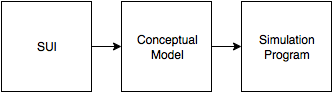
\includegraphics[height=1in,width=3.6in]{sui_mod_sim} 
			\caption{The role of the conceptual model\label{fig:01}} 
		\end{center} 
	\end{figure}
	
	\subsection{Objective}
	For this project, the objective is to model the egress of pedestrians from a stadium (Georgia 
	Tech's Bobby Dodd Stadium). The conceptual model must be generated to represent the SUI which 
	is the pedestrian movements.
	
	\subsection{Input}
	Model inputs includes pedestrian and map information. The number of pedestrians and their 
	characteristics: travel speed and destination. The simulation environment (walkways, 
	destinations, etc.) must be input as map information. The map information should be input as a 
	grid (for the CA implementation). It must contain definitions of walkways, destinations, 
	stadium exits, and street crossings (crossings can be turned on and off).
	
	\subsection{Output}
	The model output is the simulated egress of the pedestrians (given in the input) through the 
	modeled environment (map information given as an input).	
	
	\subsection{Content}
	The model does not include activities inside the stadium; however, the stadium exits do 
	provided inputs to the simulation. Therefore, the stadium and activities within are regarded as 
	exogenous entities for this model. The stadium (Bobby Dodd Stadium) can hold 55,000 spectators 
	\cite{Dodd:Misc} which provides an upper limit on the number of spectators to include in the 
	simulation. \\
	
	\noindent
	The endogenous entities in this model are pedestrians and map objects (walkways, streets, 
	etc.). A queuing model is for the pedestrian entities. They are then placed into the model as 
	space opens up at exit locations (previous pedestrians walk away). Pedestrian entities contain 
	properties for waking speed and selected destination. The walking speed distribution is 
	obtained from research in \cite{young1999evaluation} and is similar to that used in 
	\cite{burstedde2001simulation}. The walking speeds for each pedestrian 
	are drawn form the normal distribution shown in Table \ref{tbl:01}.
	
	\begin{table}[H]
		\centering
		\caption{Pedestrian Walking Speed Distribution \cite{young1999evaluation}}
		\label{tbl:01}
		\begin{tabular}{l|ll}
			& ft/sec & m/sec \\ \hline
			Mean      & 4.40   & 1.340 \\
			Std. Dev. & 0.87   & 0.265
		\end{tabular}
	\end{table}
	add note about minimum speed 0.153 m/s
	
	\noindent
	Map information is represented as a grid of cells that measure $0.21 m^2$ ($0.457 m$ sides) 
	\cite{blue2001cellular}. Each cell is given a type that represents information relevant to this 
	simulation. More specifically, the cells are identified as walkways, crosswalks, streets, or 
	prohibited.\\
	
	\subsection{Assumptions and Simplifications}
	Pedestrian entities are assumed to always travel toward their predetermined destination (they 
	do not change destinations during the simulation) and to stay on the allowed paths. The 
	pedestrian model does not include personal attributes, although some attributes may correlate 
	with pedestrian walking speed, this is taken into account through the walking speed 
	distribution. Additionally, directional travel is not modeled. Only movements directly to cells 
	that share a side with the current cell are allowed (North, South, East, and West).\\
	
	\noindent
	The map information is simplified to a 2-D grid (for use with CA). Terrain attributes (incline, 
	material, etc.) are not included.\\
	
	%%%%%%%%%%%%%%%%%%%%%%%%%%%%%%%%%%%%%%%%%%%%%%%%%%%%%%%%%%%%%%%%%%%%%%%%%%%%%%%%%%%%%%%%%%%%%%%%
	\section{Simulation Development}
	Pedestrian movement is a dynamical system and for this project, pedestrian egress from a 
	stadium, it will be modeled as a discrete time dynamical system using CA. The simulation grid 
	is made up of cells that are either ``allowed'' or ``prohibited'' for pedestrian traffic. A 
	``floor field'' \cite{varas2007cellular} is calculated for each destination and used to 
	influence the movement decisions of the pedestrians. The pedestrians enter the simulation at 
	the cells designated for the stadium exit(s). A simple time stepping loop (see Algorithm 
	\ref{alg:1}) is then used to move the pedestrians to their respective destinations. A high 
	level representation of the simulation algorithm is presented below (Algorithm \ref{alg:2}).
	
	\begin{algorithm}[h]
	  \DontPrintSemicolon
	  \KwData{Map information, number of pedestrians}
	  Define distribution of pedestrian speeds\;
	  Define distribution of pedestrian destinations\;
	  Create a queue of pedestrian objects\;
	  Create map object\;
	  Create separate static fields for each destination\;
	  \For{number of time steps}{
	  	pop pedestrinas off queue and place at stadium exit\;
	  	update pedestrian positions\;
	  	visualize map\;
	  }
	  \caption{High Level Simulation Algorithm \label{alg:2}}
	\end{algorithm}
	
	\subsection{Pedestrian Objects}
	The simulation defines a pedestrian object with the following attributes:
	\begin{enumerate}
		\item Coordinates (location on the grid)
		\item Destination ID
	\end{enumerate}
	
	\noindent
	Currently the pedestrian objects do not incorporate a speed parameter. All pedestrians are 
	assumed to have a speed of one cell per time step. This is to simplify the initial development 
	of the simulation. Eventually each pedestrian will be given a speed that is drawn from some 
	distribution.
	
	\subsection{Simulation Grid}
	A simulation grid is created to represent the desired map divided into cells. Each cell has an 
	attribute that indicates its type. A cell can have any of the types listed below.
	\begin{enumerate}
		\item Prohibited
		\item Walkway
		\item Crossing
		\item Entry point (also allowed walkway)
		\item Exit point (also allowed walkway)
	\end{enumerate}
	
	\noindent
	Using these attributes the simulation will be able to make decisions. If a cell is marked as 
	prohibited, pedestrians will not be allowed to move to those locations. Walkways and crossings 
	will be allowed. Crossing cells are identified separately so that the simulation can 
	periodically open and close the crossing to simulate real life traffic scenarios. The 
	simulation will insert and remove pedestrians at entry and exit point cells respectively.\\
	
	\noindent
	A ``floor field'' \cite{varas2007cellular} is calculated for each destination by assigning a 
	value of 1 to the destination cells and then incrementing the value of neighboring cells for 
	each step they are away from the destination. This ``field'' is used to ``force'' pedestrians 
	through the grid to their desired destination. The calculation of this field is similar to a 
	breadth-first search in graph theory and runs in $O(m+n)$ time (where $n$ is the number of gird 
	rows and $m$ is the number of grid columns). 
	
	when confronted with multiple cells of equal probability, a random choice is made
	\\
	
	\noindent
	Each cell also has attributes for the pedestrian currently occupying the cell. This provides 
	information to the movement calculations.
	
	\subsection{Pedestrian Movements (State Transitions)}
	Currently the pedestrian movements are very simple and are only influenced by the ``floor 
	field''. Next steps will involve varying speeds and collision avoidance. I don't model two way 
	traffic (since the simulation models egress only). Therefore the simulation does not include 
	``lane formation'' logic. No lanes are assumed and all pedestrians move in the same direction. 
	I need to define the function that calculates the state of a cell based on neighbors.
	
	
	
	%%%%%%%%%%%%%%%%%%%%%%%%%%%%%%%%%%%%%%%%%%%%%%%%%%%%%%%%%%%%%%%%%%%%%%%%%%%%%%%%%%%%%%%%%%%%%%%%
	\section{Description of Simulation Software}
	
	\subsection{Architecture}
	Python...
	
    \subsection{Interfaces}
    See map input data in the appendix
	
	%%%%%%%%%%%%%%%%%%%%%%%%%%%%%%%%%%%%%%%%%%%%%%%%%%%%%%%%%%%%%%%%%%%%%%%%%%%%%%%%%%%%%%%%%%%%%%%%
	\section{Simulation Results}
	The figures below show the movement of a single pedestrian along the map toward his 
	destination. Walkways are light blue and prohibited areas are dark blue. Need to show that the 
	pedestrian walking speeds are normally distributed. Show statistics on total evacuation time...
	
	\begin{figure}[H]
		\begin{subfigure}[b]{0.5\textwidth}
			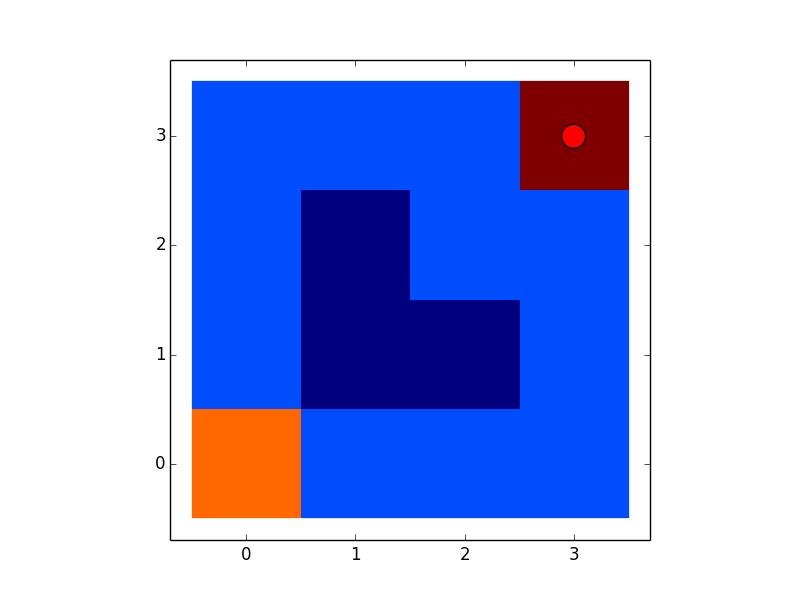
\includegraphics[width=\textwidth]{move_ex_1_step_01}
			\caption{Step 1}
			\label{fig:1}
		\end{subfigure}
		%
		\begin{subfigure}[b]{0.5\textwidth}
			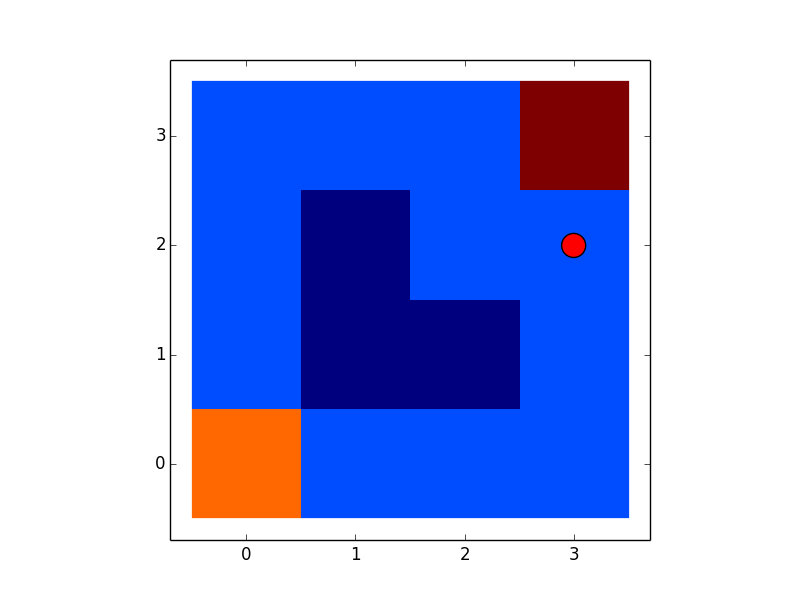
\includegraphics[width=\textwidth]{move_ex_1_step_02}
			\caption{Step 2}
			\label{fig:2}
		\end{subfigure}
		%
		\begin{subfigure}[b]{0.5\textwidth}
			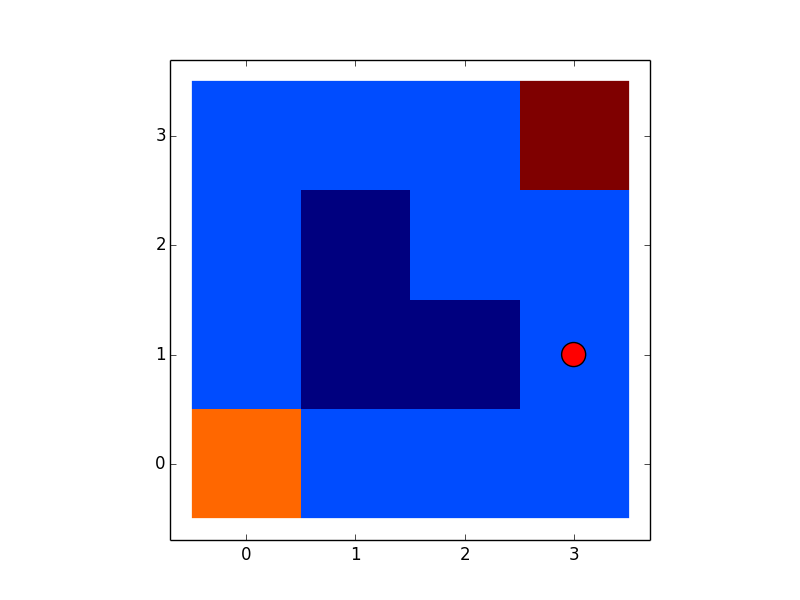
\includegraphics[width=\textwidth]{move_ex_1_step_03}
			\caption{Step 3}
			\label{fig:3}
		\end{subfigure}
		%
		\begin{subfigure}[b]{0.5\textwidth}
			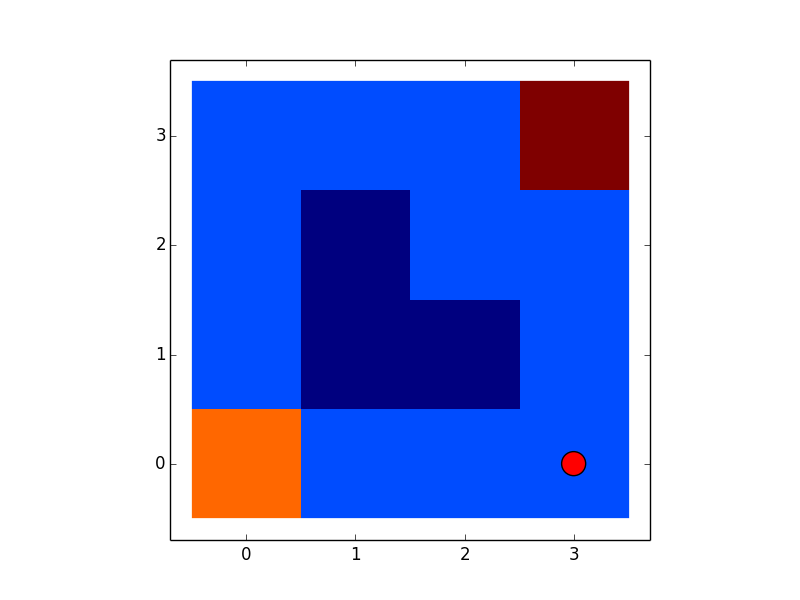
\includegraphics[width=\textwidth]{move_ex_1_step_04}
			\caption{Step 4}
			\label{fig:4}
		\end{subfigure}
		%
		\begin{subfigure}[b]{0.5\textwidth}
			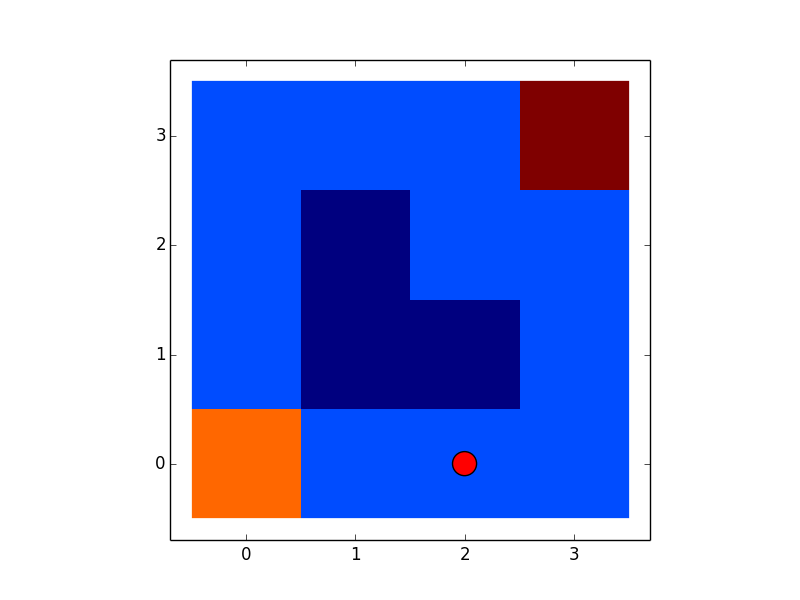
\includegraphics[width=\textwidth]{move_ex_1_step_05}
			\caption{Step 5}
			\label{fig:5}
		\end{subfigure}
		%
		\begin{subfigure}[b]{0.5\textwidth}
			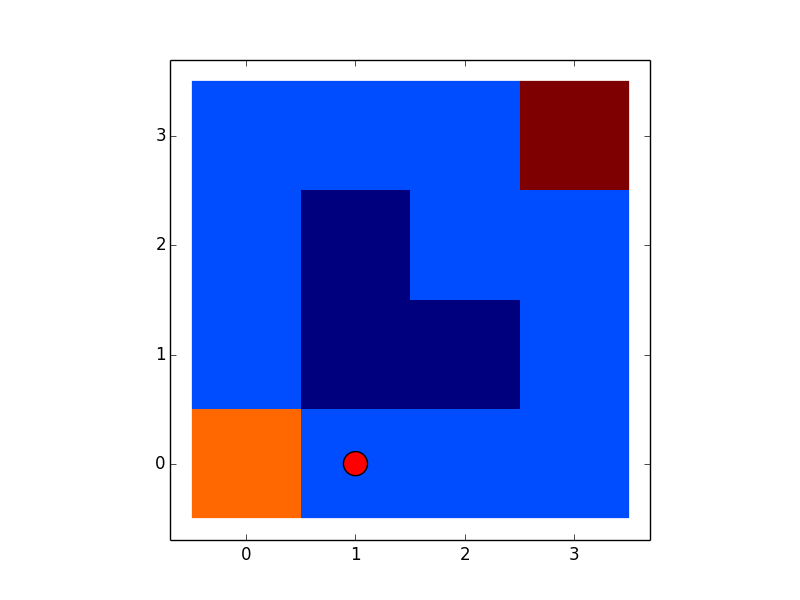
\includegraphics[width=\textwidth]{move_ex_1_step_06}
			\caption{Step 6}
			\label{fig:6}
		\end{subfigure}
	\end{figure}
	
	%%%%%%%%%%%%%%%%%%%%%%%%%%%%%%%%%%%%%%%%%%%%%%%%%%%%%%%%%%%%%%%%%%%%%%%%%%%%%%%%%%%%%%%%%%%%%%%%
	\section{Summary}
	TODO
	
	%%%%%%%%%%%%%%%%%%%%%%%%%%%%%%%%%%%%%%%%%%%%%%%%%%%%%%%%%%%%%%%%%%%%%%%%%%%%%%%%%%%%%%%%%%%%%%%%
	%%% Appendices
	\newpage
	\begin{appendices}
		\section{Map File Format}
		A custom map file format was developed for getting map information into the simulation. The 
		format defines a grid on the first row and then allows blocks of cells to be given a type 
		attribute. The simulation assumes any cells not specified to be prohibited. An example map 
		file and its corresponding map (from the simulation) are shown below. 
		
		\begin{verbatim}
		# Test Map File
		#
		# Grid size (row,col) and size of cell area (arbitrary area unit)
		100 100 1
		# Define a block (start_row,start_col) to (stop_row,stop_col) of type t
		# Cell types:
		# 0       = Prohibited (default)
		# 1       = Walkway
		# 2       = Street
		# 4       = Crossing (can also be defined by overlapping 1 and 2)
		# 3 to 99 = Arbitrary (for specific use by simulator if needed)
		# 1XX     = Destination (can be multiple destinations)
		# 2XX     = Starting location (can be multiple starting points)
		45 00 50 99 1
		00 00 99 05 1
		00 48 45 50 1
		00 00 02 50 1
		00 09 99 19 2
		00 60 99 70 2
		00 00 00 05 100
		00 00 05 00 100
		99 00 99 05 101
		45 98 50 99 200
		\end{verbatim}
		
		\begin{figure}[H]
			\begin{center} 
				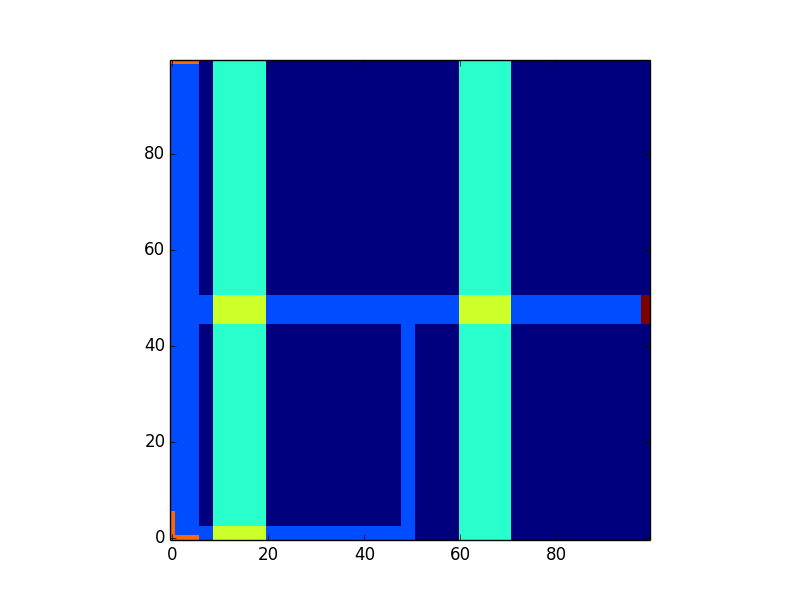
\includegraphics[height=4in,width=5.5in]{map_test_02} 
				\caption{Example map read from data file\label{fig:A:1}} 
			\end{center} 
		\end{figure}
		
	\end{appendices}  
	
	%%%%%%%%%%%%%%%%%%%%%%%%%%%%%%%%%%%%%%%%%%%%%%%%%%%%%%%%%%%%%%%%%%%%%%%%%%%%%%%%%%%%%%%%%%%%%%%%
	%%% Bibliography
	\newpage
	\bibliography{cse6730_project1_dcrocker3_report} 
	\bibliographystyle{ieeetr}
	
%%%%%%%%%%%%%%%%%%%%%%%%%%%%%%%%%%%%%%%%%%%%%%%%%%%%%%%%%%%%%%%%%%%%%%%%%%%%%%%%%%%%%%%%%%%%%%%%%%%	
%%% End document
\end{document}
